\chapter{Mobile Application Design}
\label{chap:mobile_app}

The WattMate mobile application was developed as a lightweight Android interface for  demonstrating and controlling the embedded device WattMate through BLE. The goal of the application is not to replace a production-grade mobile client, but to provide a practical interface for connection management, live telemetry visualization, stream control, and battery configuration during the project validation phase.

The application was implemented using MIT App Inventor. This choice allowed rapid development of a functional BLE-enabled prototype without introducing the additional complexity of a native Android implementation. Since the main focus of the project is the embedded system, App Inventor was considered suitable to validate the BLE protocol, test the firmware behavior, and provide a usable demonstration interface.

\begin{figure}[H]
	\centering
	% Replace with MIT App Inventor logo or development environment screenshot
	
\includegraphics[width=0.35\textwidth]{figures/AppInventor_logo.png}
	\caption{MIT App Inventor environment used for the WattMate mobile application.}
	\label{fig:appinventor_logo}
\end{figure}


\section{Application Objectives}
\label{sec:app_objectives}

The mobile application was designed around three main objectives.

\begin{itemize}
	\item \textbf{BLE connectivity management.}
	The application allows the user to scan for nearby BLE devices, select WattMate, establish a connection, disconnect, and attempt reconnection without restarting the app.
	
	\item \textbf{Live data visualization.}
	The application displays the measurements and battery statistics produced by the firmware, including electrical data, temperature, State of Charge, State of Health, and status information.
	
	\item \textbf{Device control and configuration.}
	The application can send control and configuration commands to the firmware, such as enabling or disabling the BLE data stream, resetting battery data, and configuring the nominal battery energy used by the estimation logic.
\end{itemize}

The application therefore acts as a practical bridge between the embedded firmware and the user. It does not replace the firmware logic, but exposes the most relevant firmware states and commands through a simple Android interface.


\section{Application Structure}
\label{sec:app_structure}

The mobile application is organized as a single-screen MIT App Inventor project. 
Instead of using multiple App Inventor screens, the interface is divided into visual layouts that are shown or hidden according to the current application state. 
This choice keeps the same BLE component active during navigation and avoids recreating the BLE connection when moving between different parts of the application.

The interface is composed of following main views, with each one associated with a specific phase of the interaction with WattMate:

\begin{itemize}
	\item \textbf{Connection page.}
	The connection page is the first view shown to the user. 
	It is used to start and stop BLE scanning, display the detected nearby peripherals, and select the target WattMate device. 
	The scan results are presented directly inside the application through a touch-selectable list, without opening a separate Android selection screen. 
	For each detected device, the list shows the advertised name, the BLE address, and the received signal strength indicator (RSSI), allowing the user to identify and select the correct WattMate device more reliably. 
	This page is mainly used before the BLE link is established or when the user wants to choose a different device.
	
	\begin{center}
		\captionsetup{type=figure,width=0.70\textwidth,font=small}
		
		\begin{minipage}{0.30\textwidth}
			\centering
			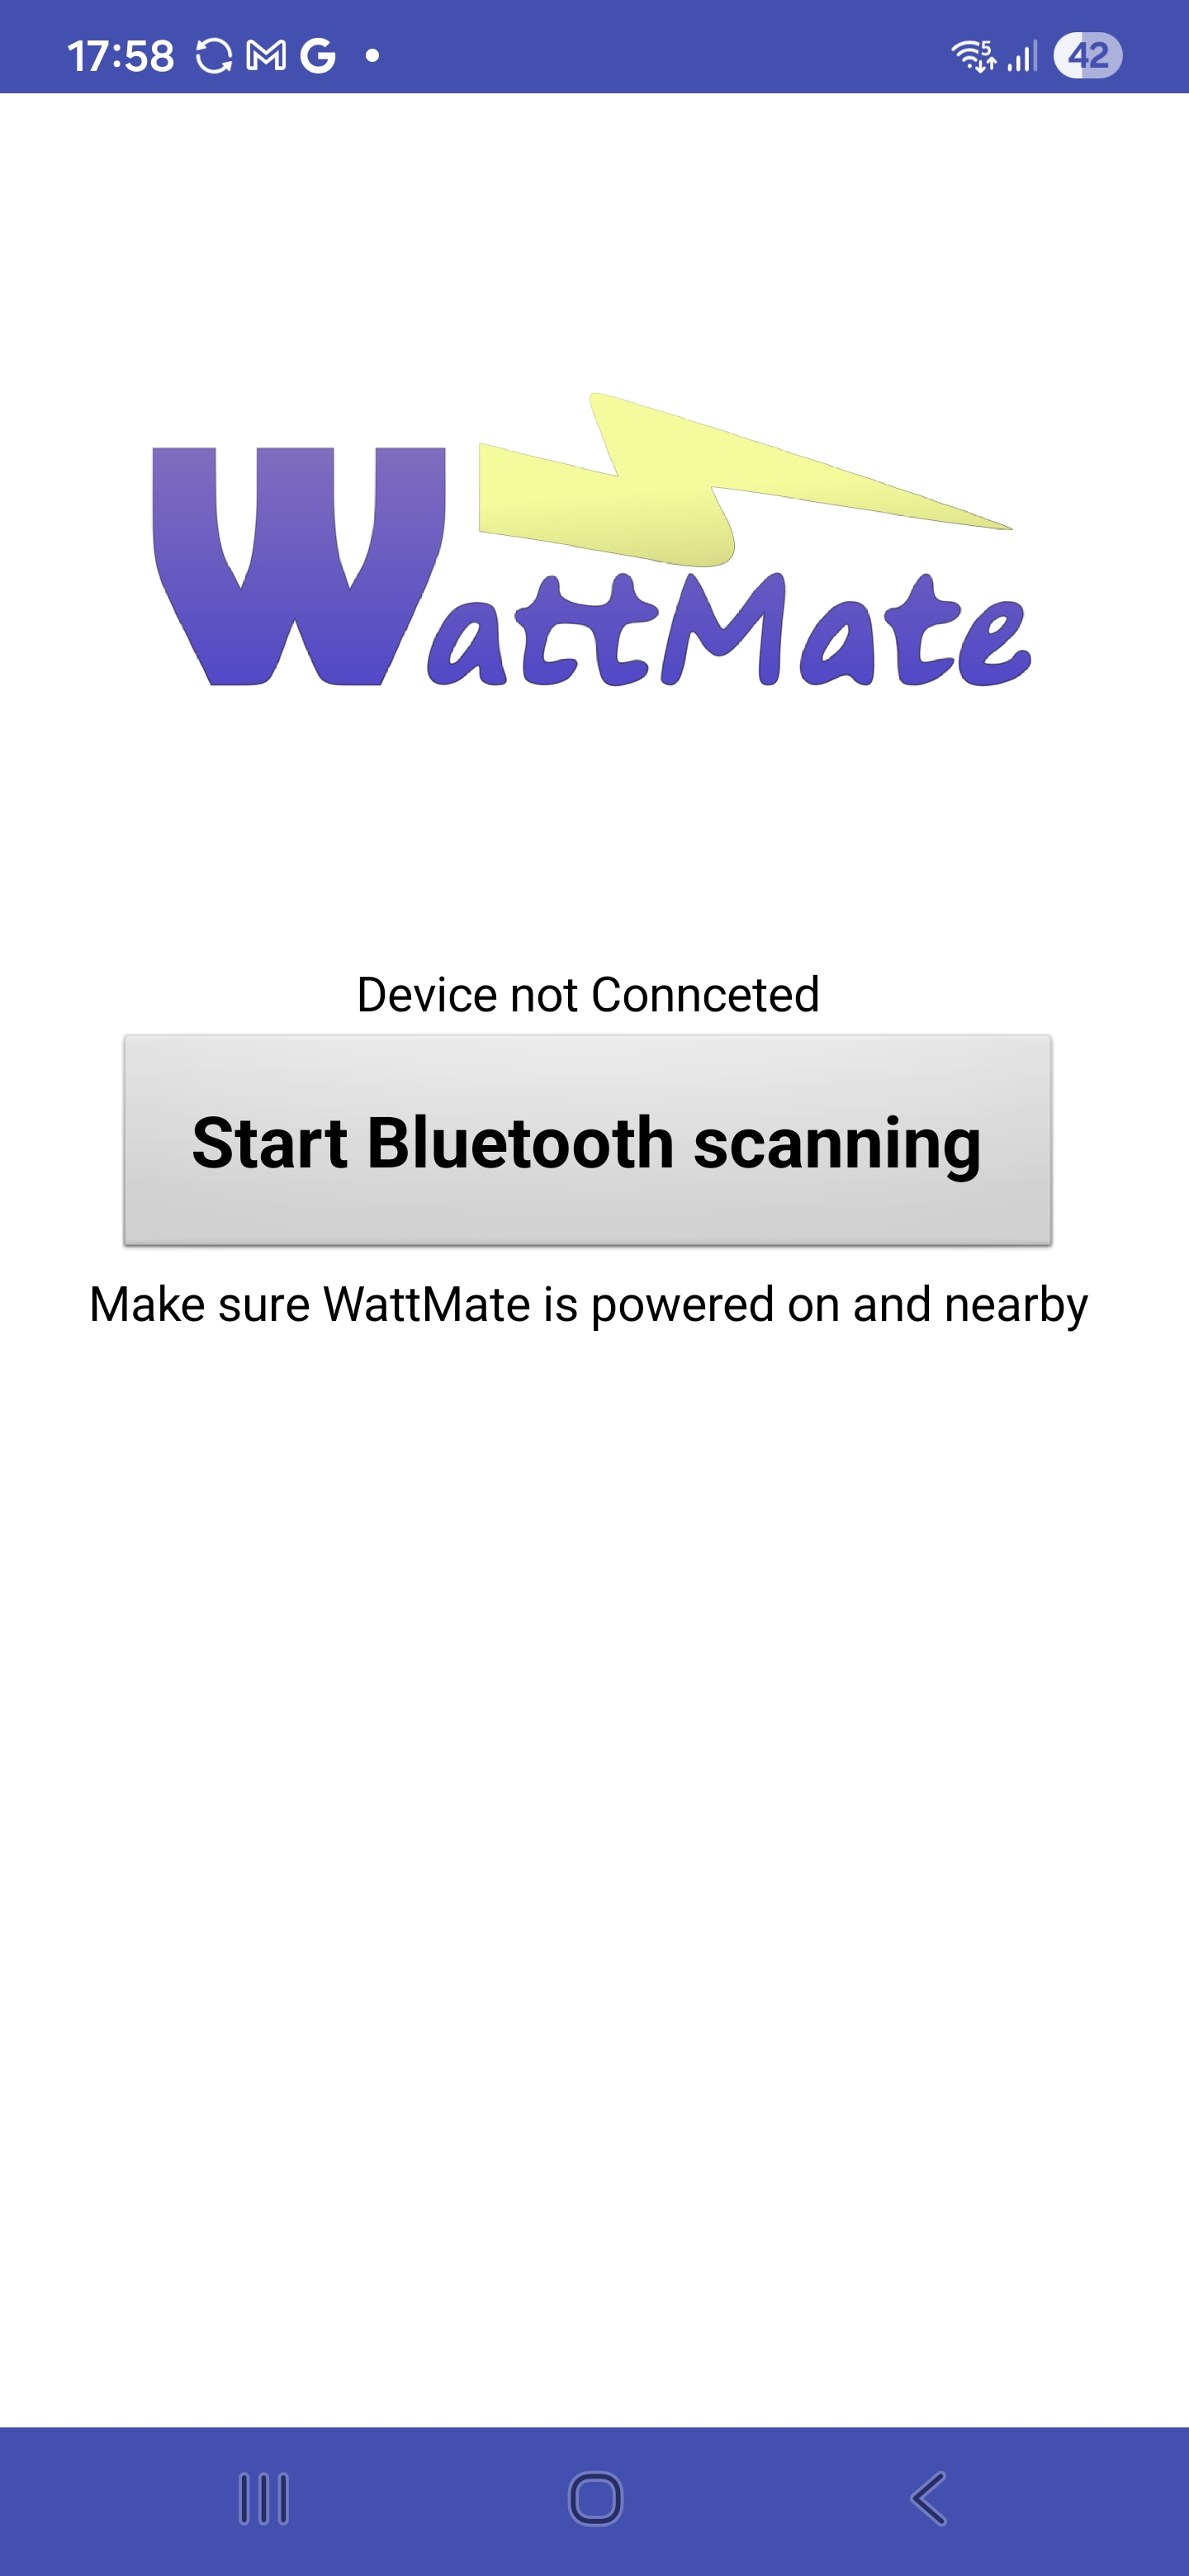
\includegraphics[width=\textwidth]{figures/3_FW_Figures/ConfigPage.jpg}
		\end{minipage}
		\hspace{1.2cm}
		\begin{minipage}{0.30\textwidth}
			\centering
			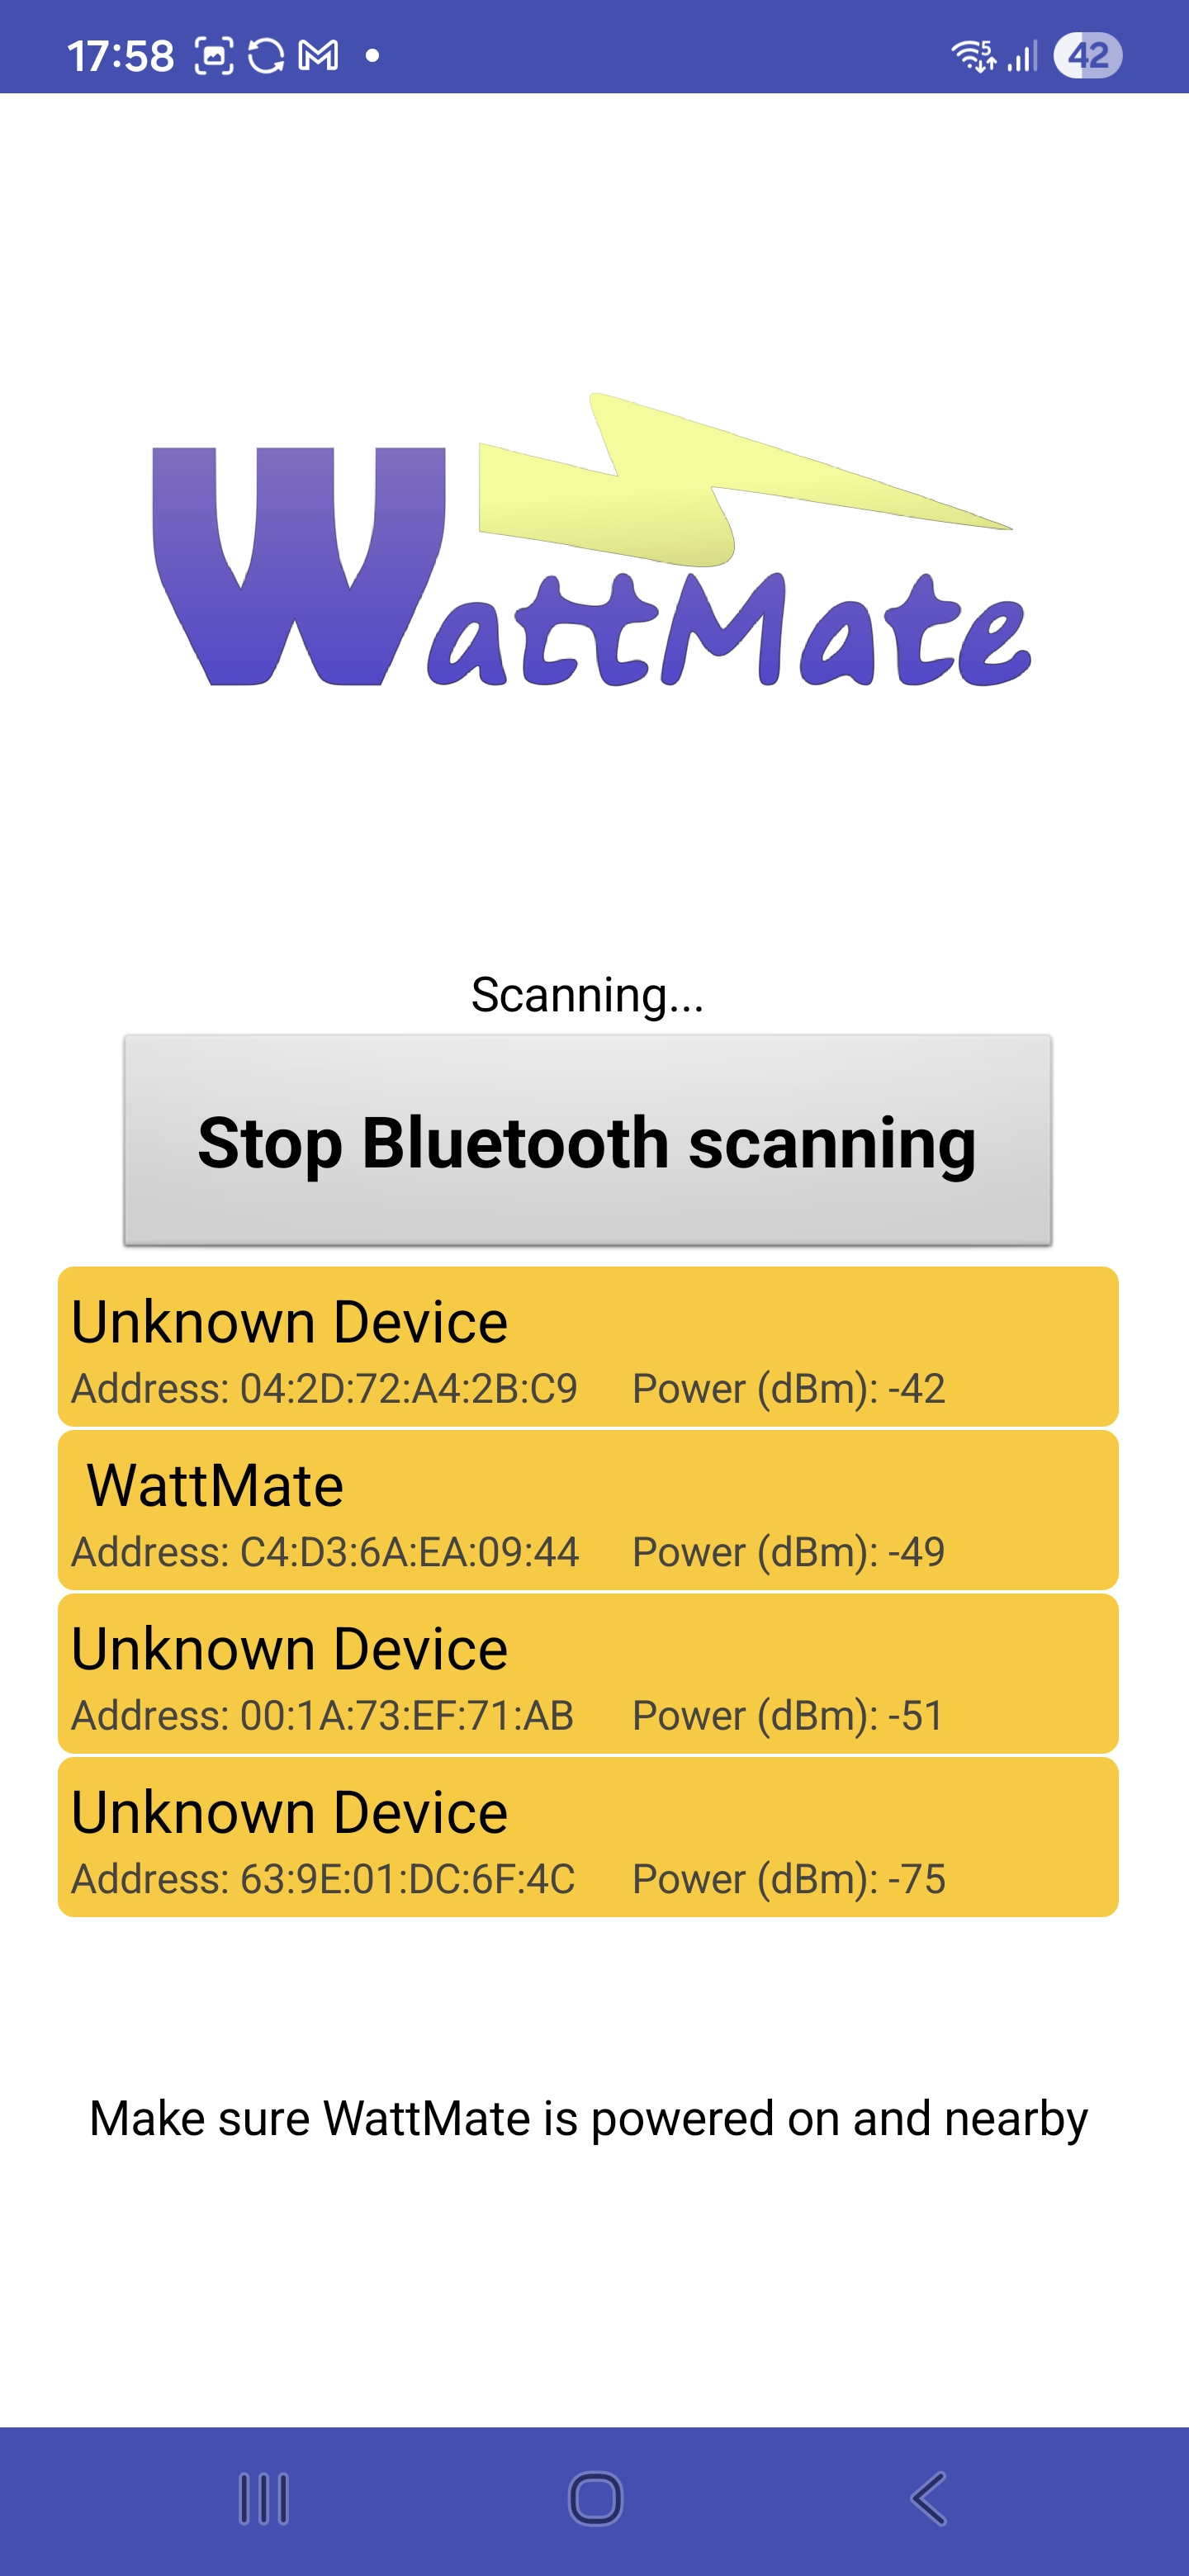
\includegraphics[width=\textwidth]{figures/3_FW_Figures/ConfigPage_BLEsearch.jpg}
		\end{minipage}
		
		\captionof{figure}{Connection page before and after pressing the "Start Bluetoth Scanning" button}
		\label{fig:App_SearchPage}
		
	\end{center}
	
	\item \textbf{Dashboard page.}
	The dashboard page is shown after a successful BLE connection. 
	It is the main view of the application and displays the connection state, the telemetry stream state, the latest update time, and the measured quantities received from WattMate. 
	It also contains the controls used to start or pause the telemetry stream, disconnect and reconnect to WattMate, or return to the device selection page. 
	Danger conditions detected by the firmware are shown through a dedicated warning banner, so that abnormal operating conditions are immediately visible during testing.
	
	\begin{center}
		\captionsetup{type=figure,width=0.70\textwidth,font=small}
		
		\begin{minipage}{0.30\textwidth}
			\centering
			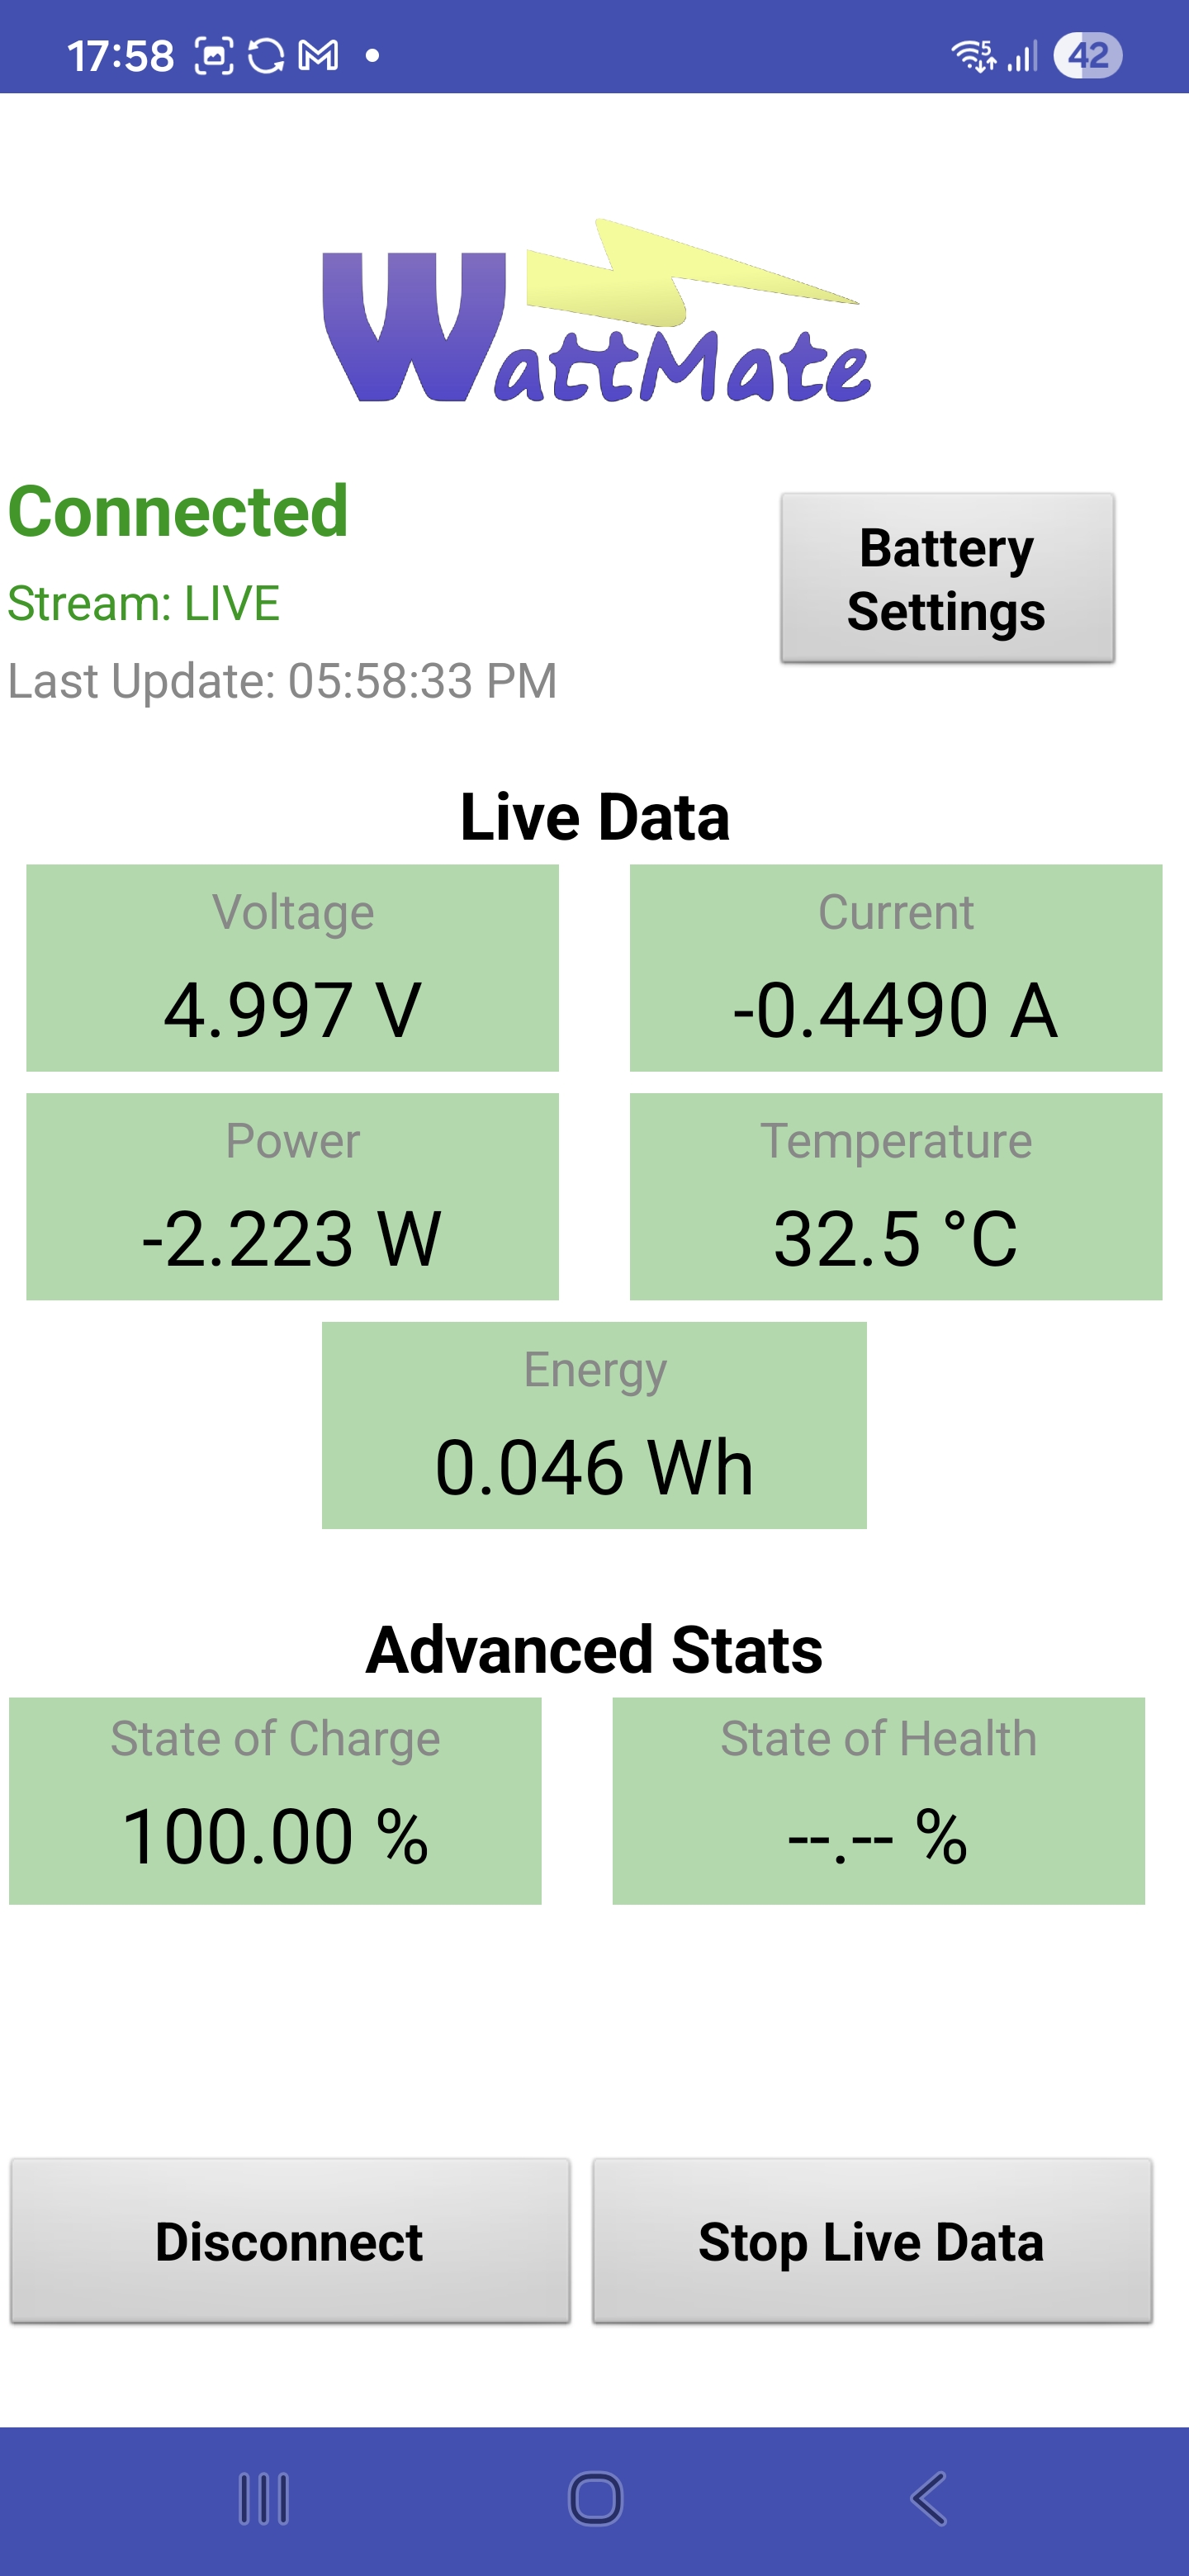
\includegraphics[width=\textwidth]{figures/3_FW_Figures/Dash.jpg}
		\end{minipage}
		\hspace{1.2cm}
		\begin{minipage}{0.30\textwidth}
			\centering
			\includegraphics[width=\textwidth]{figures/3_FW_Figures/Dash_NoStream.jpg}
		\end{minipage}
		\hspace{1.2cm}
		\begin{minipage}{0.30\textwidth}
			\centering
			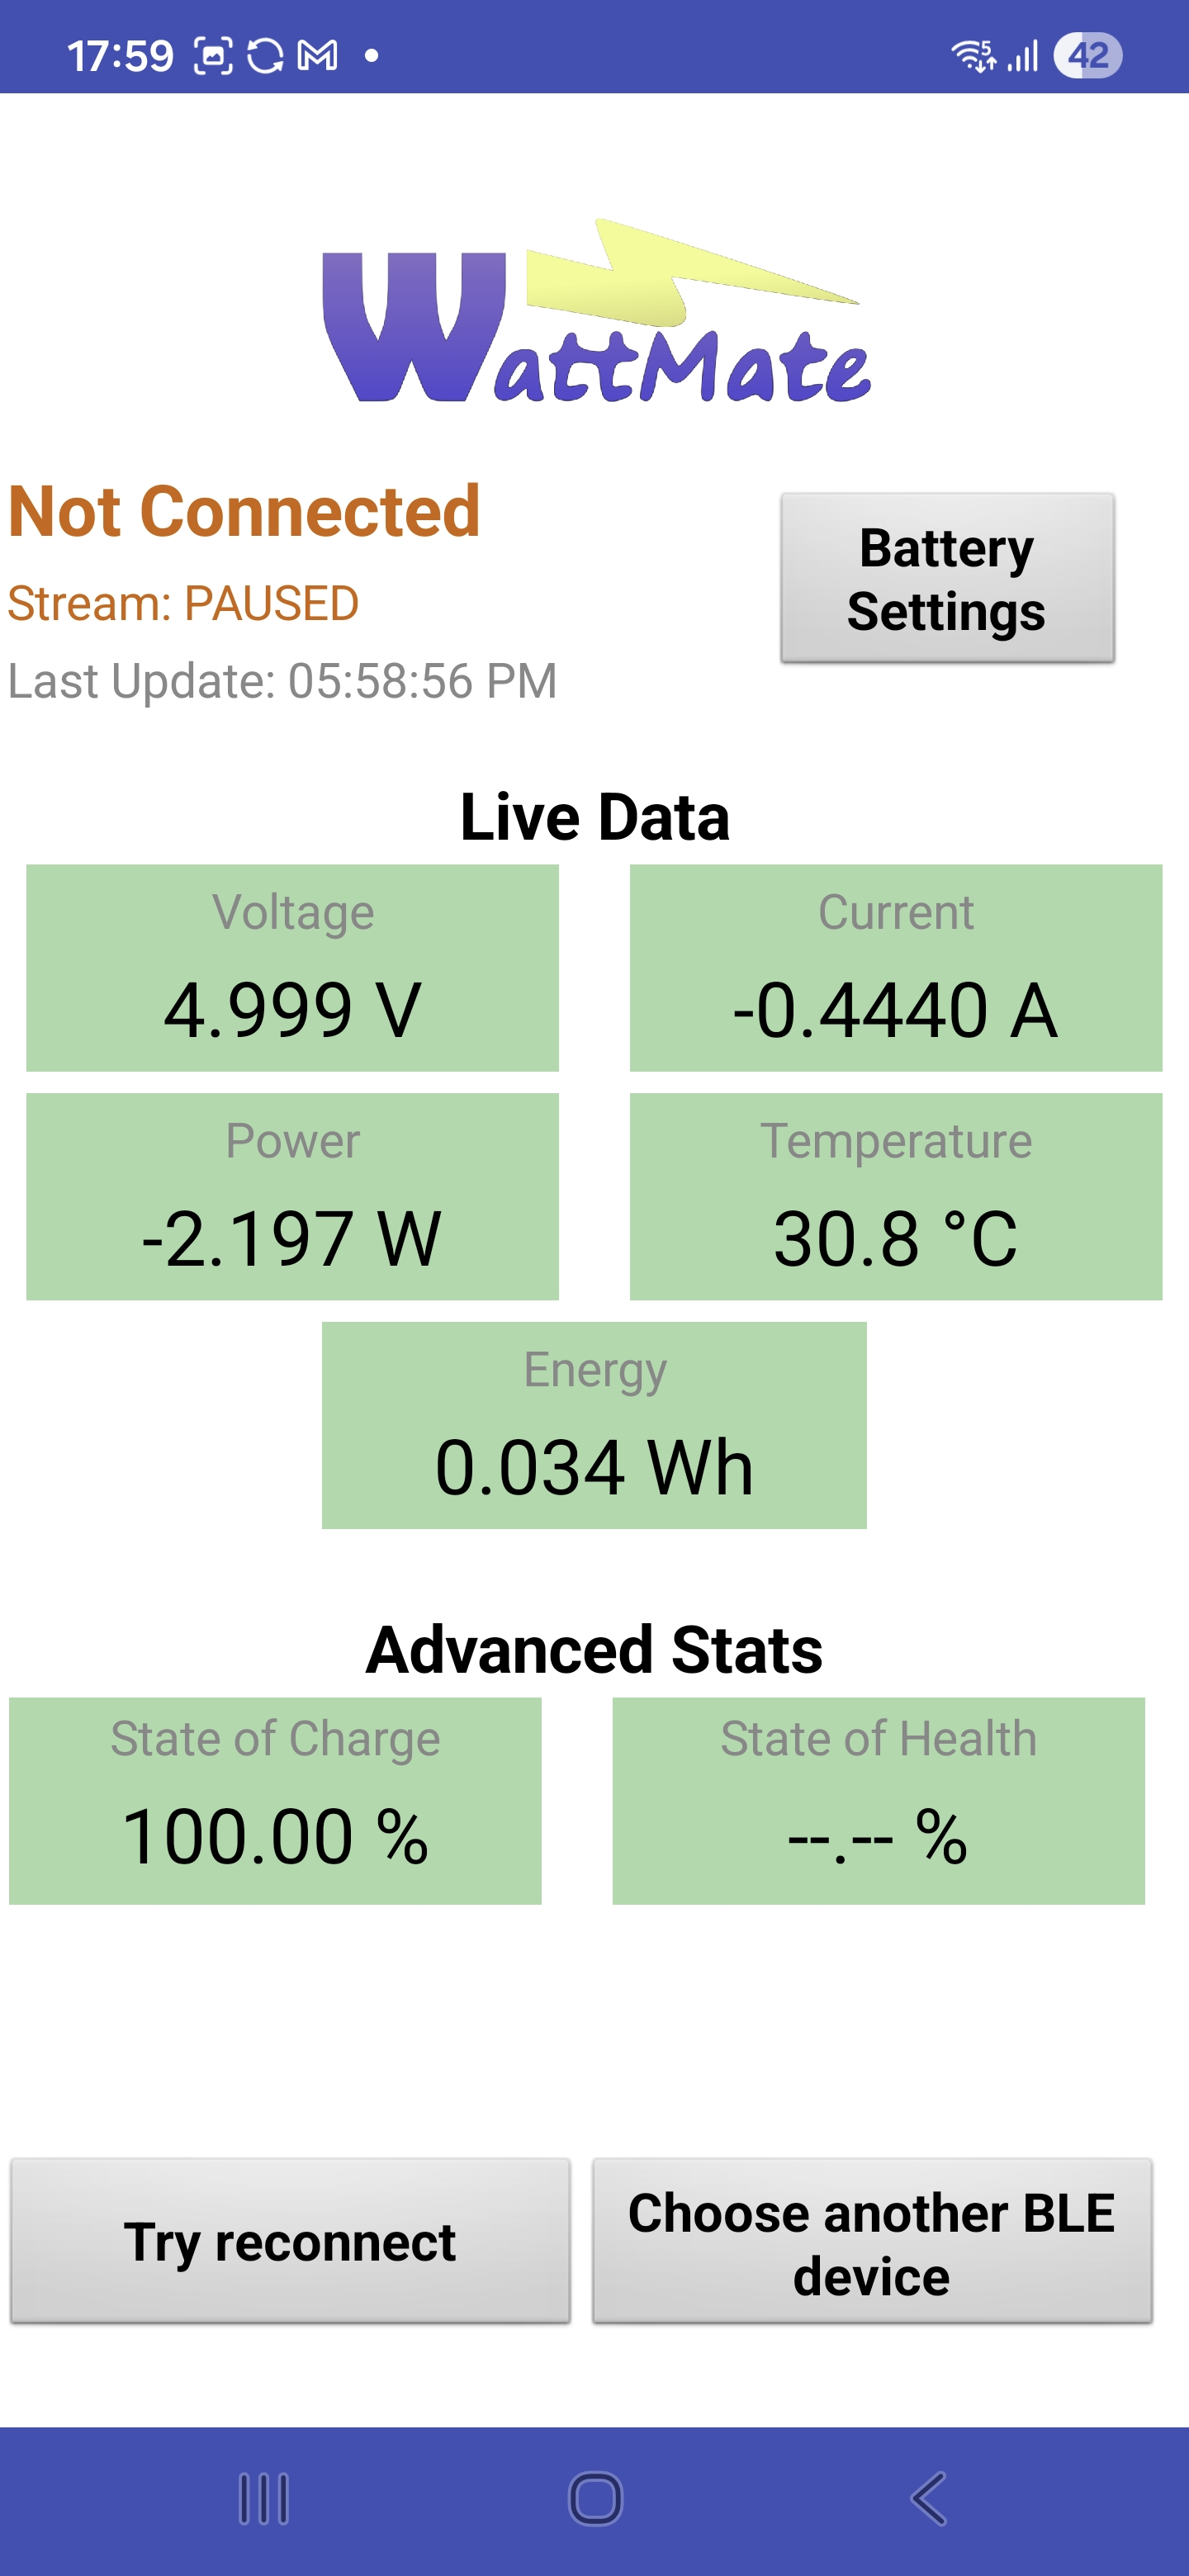
\includegraphics[width=\textwidth]{figures/3_FW_Figures/Dash_NoConn.jpg}
		\end{minipage}
		
		\captionof{figure}{Dashboard page used to display live measurements, stream state and device status}
		\label{fig:App_DashPage}
		
	\end{center}
	
	\item \textbf{Battery setup page.}
	The battery setup page is used to configure the information required by the firmware battery estimation logic. 
	The user selects the cell type from a predefined list and specifies the number of cells of that type used inside the tested power bank. 
	The application then computes the corresponding nominal battery energy and sends this value to WattMate through the dedicated BLE configuration characteristic. 
	The same page also provides a reset command to clear the stored battery estimation data, which is useful when a different battery or power bank is connected.
	
	\begin{center}
		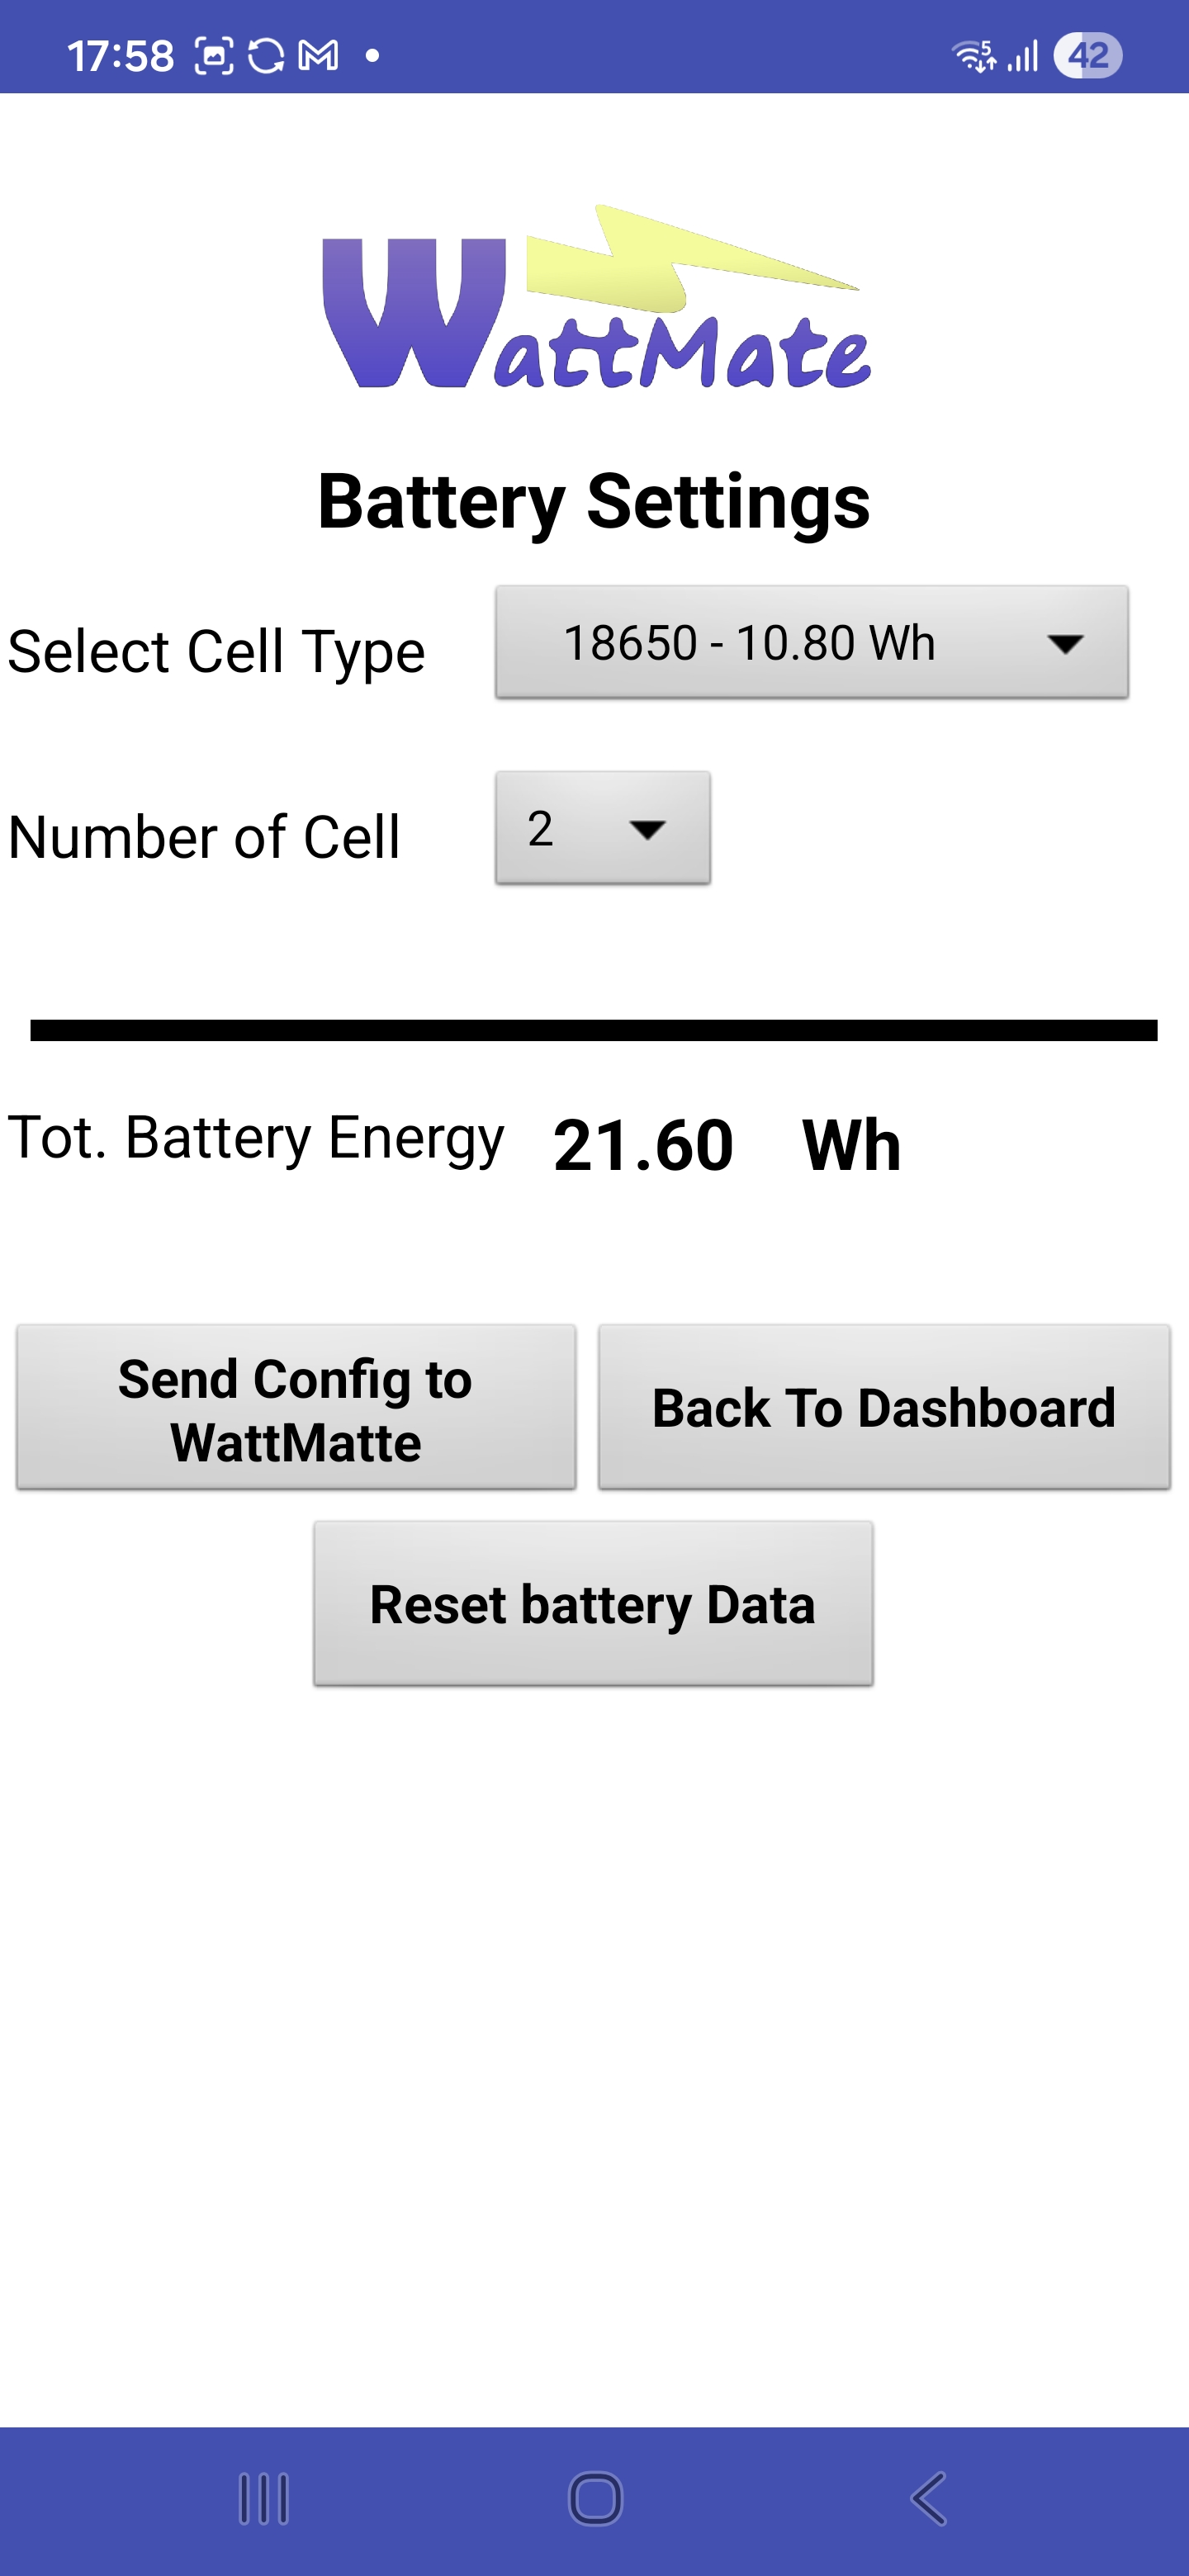
\includegraphics[width=0.30\textwidth]{figures/3_FW_Figures/BatterySettings.jpg}
		\captionof{figure}{Battery settings page, used to send the current battery setup to WattMate}
		\label{fig:App_BatterySettingsPage}
	\end{center}
\end{itemize}

This organization keeps the interface readable while preserving a simple internal structure. 
All views belong to the same App Inventor screen, and navigation is implemented only by changing the visibility of the corresponding layouts. 
This approach is sufficient for the prototype application and reduces the risk of losing the BLE state during navigation.

\section{BLE Communication Interface}
\label{sec:app_ble_interface}

The mobile application communicates with WattMate through the custom BLE service exposed by the firmware, whose structure is described in Table~\ref{tab:ble_custom_service}. 
In this chapter, the BLE interface is considered from the application side, focusing on how the Android client interacts with the characteristics published by WattMate.

After a connection is established, the application behaves differently depending on the type of characteristic exposed by the firmware:

\begin{itemize}
	\item \textbf{Notification characteristics.}
	Characteristics used for firmware-to-app data transfer are handled through BLE notifications. 
	The application must explicitly subscribe to these characteristics before receiving updates. 
	Once the subscription is active, the firmware can push new binary payloads to the phone without requiring repeated read requests from the app. 
	This mechanism is used for live telemetry, temperature updates, and battery status information.
	
	\item \textbf{Write-only characteristics.}
	Characteristics used for app-to-firmware communication are accessed through BLE write operations. 
	In this case, the application sends short binary payloads to request high-level actions or to transfer configuration values. 
	This mechanism is used to enable or disable the data stream, reset stored battery data, and send the nominal battery energy configured by the user.
\end{itemize}


\section{Connection and Stream Management}
\label{sec:app_connection_stream}

The application explicitly separates the BLE connection state from the telemetry stream state. 
A connected device is not required to continuously send telemetry notifications. 
After the BLE link has been established, the user can independently enable or disable the data stream through the control characteristic.

This separation is useful because WattMate can remain connected without continuously transmitting live measurement data. 
When the stream is disabled, the BLE link application-level traffic is reduced to the minimum required to maintain the connection. 
This significantly reduces the amount of data transmitted by the device and avoids unnecessary telemetry notifications when live values are not needed.

In the prototype application, stream control is exposed to the user through a dedicated button. 
This makes the behavior explicit during testing and allows the BLE protocol and firmware logic to be validated directly. 
In a more complete product implementation, the same mechanism could be handled automatically by the application. 
For example, the stream could be disabled when the user moves to a non-dashboard section of the app or when the app is moved to the Android background.

The current implementation does not include automatic background management, mainly because handling Android background execution would add complexity outside the main scope of the project. 
However, the implemented manual control demonstrates the required BLE and firmware functionality: the mobile application can keep the device connected while independently requesting or stopping the live telemetry stream.

\section{Displayed Data and Battery Information}
\label{sec:app_displayed_data}

The values shown by the application are directly obtained from firmware notifications. Electrical quantities are received through the telemetry characteristic, while temperature and battery status information are received through dedicated characteristics. The app only performs unit conversion and formatting.

The data received through BLE also include danger flags generated by the firmware. 
These flags are used to indicate abnormal operating conditions, such as overvoltage, overcurrent, or overtemperature. 
When at least one danger condition is active, the application displays a dedicated warning banner on the dashboard, making the condition clearly visible during testing.

It must be noted that the visualization of a danger condition on the mobile application is limited by the BLE telemetry update period. 
In the current implementation, telemetry packets are sent every \(500\,\mathrm{ms}\), so the warning banner can be updated with the same order of delay. 
This delay is acceptable for the mobile interface, because the application is only used to present the system state to the user. 
The user is not expected to take immediate safety-critical decisions based on the app visualization.

Fast reaction to abnormal operating conditions must instead be handled locally by the firmware and by the available hardware resources. 
For this reason, the danger banner should be considered a diagnostic and user-feedback feature, while the actual protection logic belongs to the embedded device.

Another interesting point is the fact that battery-related quantities are displayed together with their validity or estimation status when available. In particular, depending on the internal firmware state, the SoC, SoH and Session Energy can be unavailable, estimated, or based on a learned battery reference, as described in Section \ref{Main_Application_Task}.


\section{Battery Configuration and Control Commands}
\label{sec:app_battery_config_commands}

The mobile application is also used to send configuration and control information to the firmware. These messages are intentionally high-level: the application does not directly modify firmware internals, but requests actions that are then interpreted and applied by the embedded software.

The main configuration value sent by the app is the nominal battery energy. This value is computed from the selected cell type and the number of cells configured in the battery setup page. It is then sent to the firmware through the battery configuration characteristic. The firmware can use this value as a nominal reference for the battery total energy.

Control commands are sent through the control characteristic. They are used to enable or disable the telemetry stream and to request a full battery data reset. The reset command is intended for cases where the tested battery or power bank is replaced, so that previously learned battery information is no longer valid.

\begin{table}[H]
	\centering
	\small
	\caption{Main commands sent by the mobile application.}
	\label{tab:mobile_app_commands}
	\begin{tabularx}{\textwidth}{lX}
		\toprule
		\textbf{Command} & \textbf{Purpose} \\
		\midrule
		
		Start stream &
		Request periodic BLE telemetry notifications. \\
		
		Stop stream &
		Stop periodic BLE telemetry notifications while keeping the BLE connection active. \\
		
		Configure nominal energy &
		Send the nominal battery energy used by the firmware as battery reference. \\
		
		Reset battery data &
		Request the firmware to clear the stored battery estimation history, for example after replacing the battery or power bank. \\
		
		\bottomrule
	\end{tabularx}
\end{table}